%!TEX root = ../thesis.tex
% ******************************* Thesis Appendix C ********************************

\ifpdf
\graphicspath{{Appendix3/Figs/Raster/}{Appendix3/Figs/PDF/}{Appendix3/Figs/}}
\else
\graphicspath{{Appendix3/Figs/Vector/}{Appendix3/Figs/}}
\fi
\chapter{Software Descriptions}
\label{sec:software_descr}

\section{Costanza}
\label{sec:costanza}
Costanza (COnfocal STack ANalyZer Application)~\cite{costanza} is an ImageJ plugin for
segmenting compartments in the form of cells and extract quantitative data,
including intensities. Primarily, Costanza is used to segment nuclei marked
cells in three dimensions and effectively extract information relating to the
intensity of the used GFP markers.

The software utilises a steepest gradient ascent approach for segmentation, which
initiates at each voxel in the stack and attempts to find local intensity maxima
by ascension in the neighbourhood of the voxel. All paths leading to the maximum
are then grouped and recorded as a Basin Of Attraction (BOA), i.e.\ cell. In the event that
multiple neighbourhood voxels have a higher intensity than the current one, the
path with the highest ratio of intensity difference over spatial difference is
chosen, i.e.\ the path returning $max\left( \frac{\Delta I}{\Delta \bar x} \right)$.

Costanza performs preprocessing in the form
of intensity inversion, background extraction and applied denoising filters. 
For postprocessing, it allows for Basin-Of-Attraction (BOA) removal and merging, in
order to exclude misidentified cells in the background and avoid faulty
separation of individual cells. 

% Say something about parameters?
% Where should citation(s) go?

\section{MARS-ALT}
\label{sec:marsalt}
MARS-ALT is software developed for spatiotemportal tissue reconstruction and lineaging at cell
resolution. The software consist of the two parts MARS (Multi-angle image
Acquisition, 3D Reconstruction and cell Segmentation), and ALT (Automated Linage
Tracking). It works by importing fluorescently stained confocal images, and
(optionally) correcting these using low-resolution reference stacks. 

For cell segmentation, MARS denoises the image using an alternate sequential filter in
order to increase the signal / noise ratio. Seeds are then extracted by
computing voxel minima, and merging those that have a lower largest valley
between them than some defined value. The background is then extracted from the
largest connected component found in the image after thresholding. Cells are
thereafter watershed using the seeds as references, with cell volumes less than
some specified value are filtered. Markers are subsequently removed from the
seeds, and the watershed algorithm is repeated until
convergence~\cite{fernandez2010imaging}.

\section{Organism}
\label{sec:organism}
Organism is C++ software for simulating biological systems, in particular with
multiple compartments primarily in the form of cells. It includes both
biochemical and mechanical rules, including rules for proliferation, for
numerically simulating the system. Organism relies on a representation of
compartments such that all of them can be described by a fixed number of
variables and parameters, such as spheres, cylinders and similar. It can also be
used for simulations of natural tissues, extracted from confocal microscopy
images. As part of the Organism toolset, software for visually inspecting
simulated tissue from output data is accessible (Newman), as well tools for
performing parameter optimisation of
GRNs~\cite{jonsson2005explicit,gruel2016epidermis}.

For this thesis, an R wrapper for interacting with parts of the Organism software was
constructed, allowing for R-based solver, model, parameter, and initialisation file setup.
Code relating to this is hosted at the \textit{Sainsbury Laboratory at the University of
  Cambridge} GitLab portal, and can be accessed at 
\url{https://gitlab.com/slcu/teamHJ/henrik_aahl/organism_wrappeR}.

\section{extractoR}
\label{sec:extractoR}
\begin{figure}[H]
  \centering
  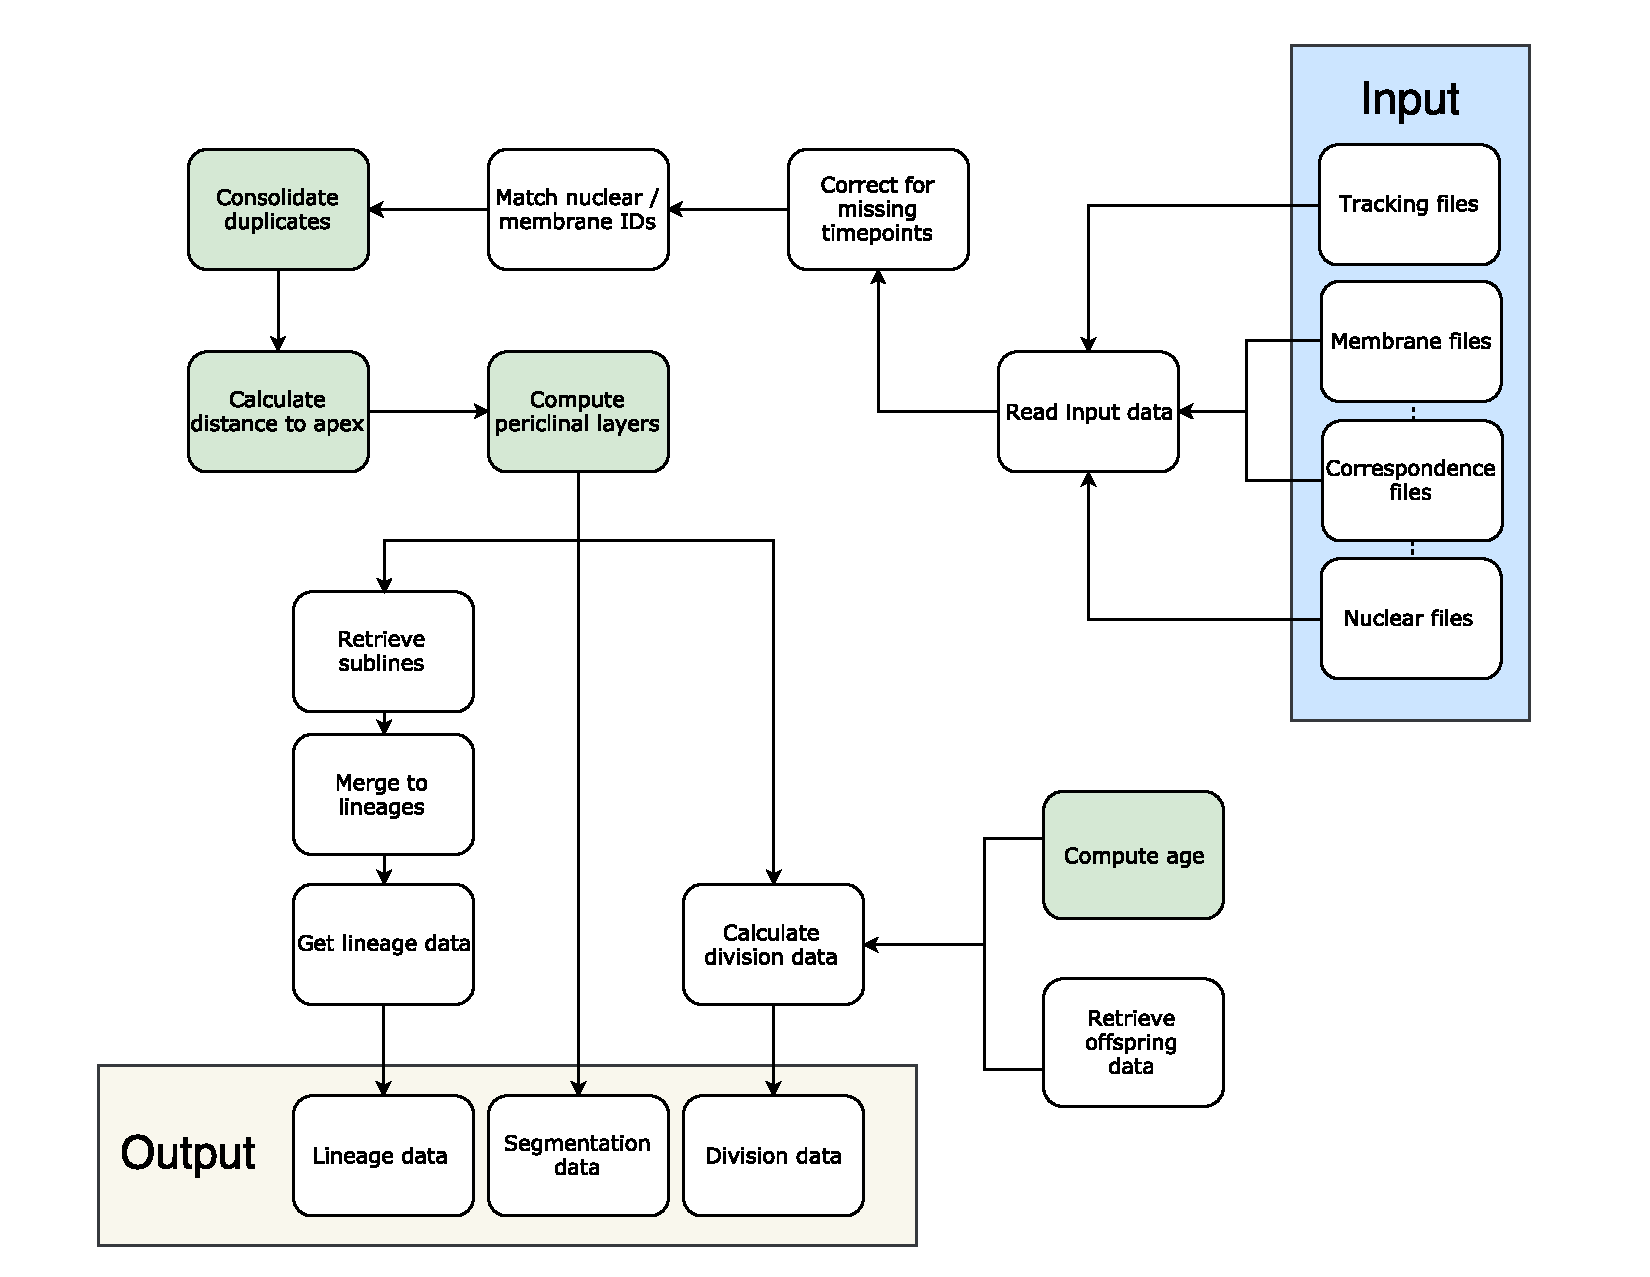
\includegraphics[trim={1.5cm 0 1.5cm .5cm}, clip, width=\textwidth]{extractor.pdf}
  \caption[extractoR flowchart]{Flowchart description of the extractoR software used within this
    study.}
  \label{fig:extractor}
\end{figure}

extractoR is convenience software developed for the data analysis part of this
thesis, with the general workflow described in \cref{fig:extractor}. The
software in developed in $R$, with minor data import scripts written in Python.
It builds on the \textit{tidyverse}, or \textit{split-apply-combine},
principle~\cite{wickham2011split} with data separated primarily into tabular
format. For convenience, extractoR
outputs the three  tabular data objects  
\begin{enumerate}
  \item Segmentation data
  \item Division data
  \item Cell line data
\end{enumerate}
all consisting of identifiers for the corresponding plant, timepoint, cell ID,
and other related metrics. The software utilises minor parallelisation in
several processing steps for optimisation purposes.
Code and related files are as of the date of
publication accessible on the SLCU GitLab page via 
\url{https://gitlab.com/slcu/teamHJ/henrik_aahl/extractoR}.

\section{TissueViewer}
\label{sec:tissueviewer}
TissueViewer is in-house software primarily developed by Yassin Refahi at SLCU. The
software provides a user-friendly visualisation tool for segmented cellular
images, and is equipped with a toolbox able to separate visualisation to select
cells, e.g.\ layer-wise. 

TissueViewer also includes the plugin Meristem Phenotyper 3D, developed by Max
Brambach at SLCU, which allows for fitting of geometric structures to raw
meristem images. In this thesis, we use this to fit paraboloid shapes to our
meristem images in order to extract information about the geometric apex, for
comparison to the one given by the gene expression.
